\documentclass{ctexart}

\usepackage{amsmath}

\usepackage{amsthm}

\usepackage{amssymb}

\usepackage{cases}

\usepackage{bm}

\usepackage{graphicx}

\usepackage{listings}
\lstset{
basicstyle=\scriptsize
}

\usepackage{caption}

\begin{titlepage}

\title{微分方程数值解 \\ 第八周作业}

\author{于慧倩 \\ 14300180118}

\date{2017年5月}

\end{titlepage}

\begin{document}

\maketitle

\newpage

\begin{enumerate}

\item P136.1

说明极值原理中的\(c(x)\)为负时,极值原理可能不成立。考虑一维的Helmholtzf方程,找u满足
\[
\frac{\mbox{d}^2 u}{\mbox{d} x^2 }+k^2 u=1, u(0)=u(1)=0\]

由课本P130知,当\(b^2+4ac \leq 0\),特别是\(b=0,ac \leq 0\)时,解是震荡的,解得Helmholtz方程的解如下:

\[u(x)=\frac{1}{k^2} ( \frac{\cos k-1}{\sin k} \sin kx-\cos kx+1)\]

\centerline{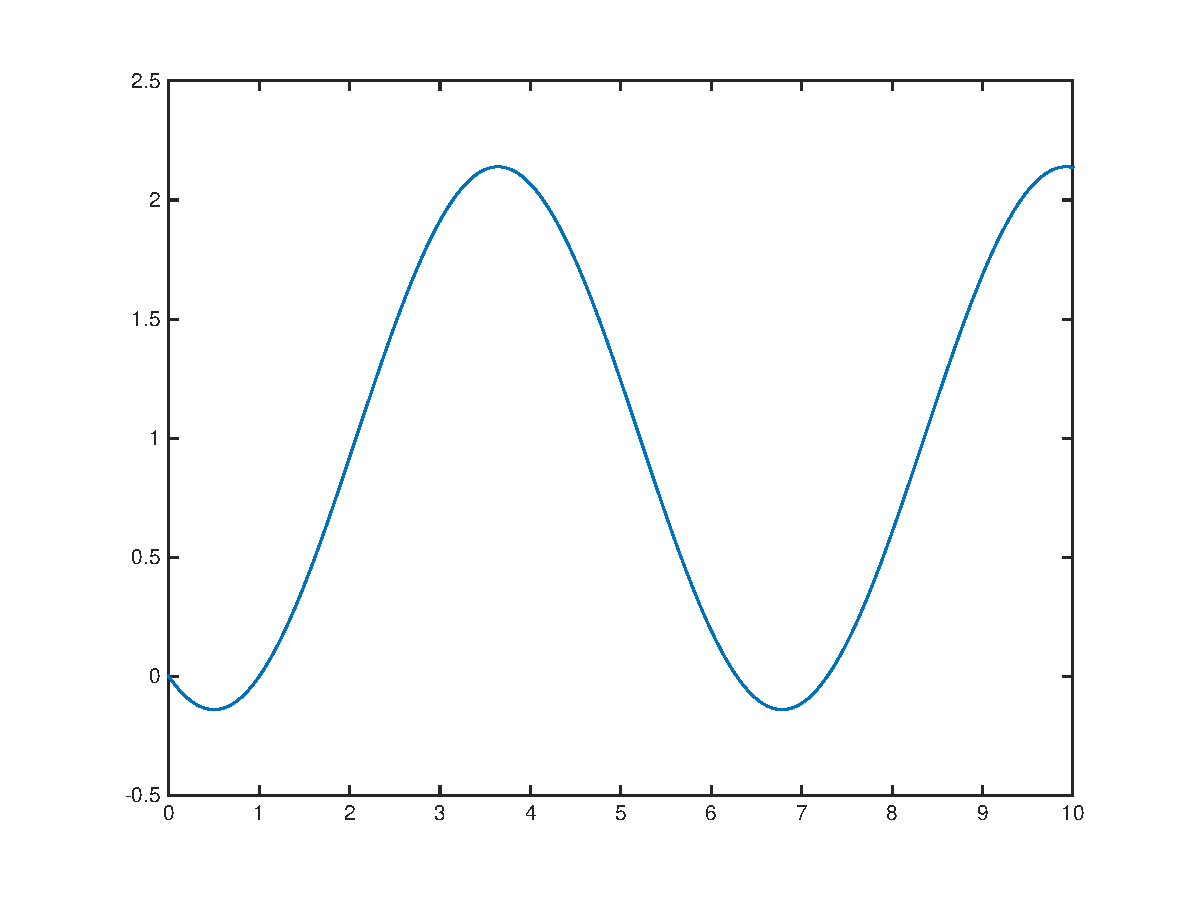
\includegraphics[width=5.5in]{H8_1_1.eps}}



\item 对初边值条件$u(0) = 0, u'(1) = 0$求相应的格林函数。

解:求解下列方程

\begin{numcases}{}
\frac{\mbox{d}^2 G}{\mbox{d} x^2} = 0, x \in (0, x_0)\cup(x_0, 1) \\
G(0) = G'(1) = 0 \\
G'_{\_}(x_0) - G'_{+}(x_0) = 1
\end{numcases}

由\((1)\)和边界条件可得:
\[
G(x,x_0) = \left\{
\begin{aligned}
&ax\quad &x<x_0\\
&b\quad &x\geq x_0
\end{aligned}
\right.
\]
由连续性得:
\[
ax_0 = b
\]
由\((3)\)得:
\[
a = 1
\]
因此有:
\[
G(x,x_0) = \left\{
\begin{aligned}
&x\quad &x<x_0\\
&x_0\quad &x\geq x_0
\end{aligned}
\right.
\]

\item P143 对方程\((3.1.3)\),如果边界条件改为\(u(0)=0, \frac{\mbox{d}u}{\mbox{d}x}(1)+u(1)=0 \),求其精确解;并用三点差分格式离散求解,同时分析差分格式的精度:

\begin{enumerate}

\item 求解精确解:

\begin{enumerate}
\item \(b=c=0\)时

 \(-au_{xx}=1\),容易得到方程解\(u(x)=-\frac{1}{a}(x-x_0)x\),由边界条件得到
 \[u(x)=-\frac{1}{a}(x-\frac{3}{2})x\]
 
 \item \(c=0,b\neq0 \)时
 
 \(-au_{xx}+bu_x=1\),此时\(u(x)=\frac{x}{b}\)是方程的一个特解,易得特征方程
 \[-a\lambda^2+b\lambda=0\]
 
 得到\(\lambda_1=\frac{b}{a},\lambda_2=0\),则有 \(u(x)=\alpha_1 e^{\frac{bx}{a}}+\alpha_2+\frac{x}{b}\)
   
由边界条件最终得到

\[
u(x)=-\frac{2}{b}\frac{1}{\lambda e^{\lambda}+e^{\lambda}-1}e^{\lambda x}+\frac{2}{b}\frac{1}{\lambda e^{\lambda}+e^{\lambda}-1}+\frac{x}{b},\lambda=\frac{b}{a}
\]

\item \( c \neq 0 , b^2+4ac > 0\)时

此时有\(\frac{1}{c}\)为一个通解,同时特征方程
\[
-a \lambda^2+b \lambda +c =0\]

有两个根\(\lambda_1= \frac{b+\sqrt{b^2+4ac}}{2a}\)和\(\lambda_2= \frac{b-\sqrt{b^2+4ac}}{2a}\),则\(u(x)=\alpha_1 e^{\lambda_1 x}+\alpha_2 e^{\lambda_2 x}+\frac{1}{c}\),同样利用边界条件得到

\[
u(x)=\frac{1}{c}\frac{-1+\lambda_2 e^{\lambda_2}+e^{\lambda_2}}{\lambda_1 e^{\lambda_1}+e^{\lambda_1}-\lambda_2 e^{\lambda_2}-e^{\lambda_2}} e^{\lambda_1 x}+\frac{1}{c}\frac{-1+\lambda_1 e^{\lambda_1}+e^{\lambda_1}}{\lambda_1 e^{\lambda_1}+e^{\lambda_1}-\lambda_2 e^{\lambda_2}-e^{\lambda_2}}e^{\lambda_2 x} +\frac{1}{c}
\]

\item \( c \neq 0 , b^2+4ac = 0\)时

有通解\(u(x)=(\alpha_1 x+\alpha_2)e^{\frac{b}{2a}x}+\frac{1}{c}\),再由边界条件得到:
\[
u(x)=( \frac{e^{\lambda}(1+\lambda)-1}{c e^{\lambda}(2+\lambda)}x-\frac{1}{c})e^{\frac{b}{2a}x}+\frac{1}{c}
\]


\item \( c \neq 0 , b^2+4ac < 0\)时

对于特征方程有共轭解\(\lambda=\alpha+\mbox{i} \beta\),所以\(e^{\alpha x} \mbox{cos} \beta x, e^{\alpha x} \mbox{sin} \beta x\)为通解,同时\(\frac{1}{c}\)为方程的。

由边界条件解得

\[
u(x)=\frac{1}{c}(\frac{-e^{-\alpha}+(\alpha+1) \mbox{cos} \beta -\beta \mbox{sin}\beta}{\beta \mbox{cos}\beta +(\alpha+1) \mbox{sin} \beta} \mbox{sin} \beta x e^{\alpha x}-\mbox{cos}\beta x e^{\alpha x}+1)
\]
\end{enumerate}

\item  用三点差分格式离散求解

方程\(3.1.3\)写作\(-\frac{\mbox{d}^2u}{\mbox{d}x^2}+\frac{b}{a} \frac{\mbox{d}u}{\mbox{d}x}+\frac{c}{a}u=\frac{1}{a} \),初值条件为\(u(0)=0,\dot{u}(1)+u(1)=0\)
用三点差分格式求解,将区间\([0,1]\)进行N等分,步长\(h=\frac{1}{N}\)。

\begin{enumerate}
\item 镜像法得到第三类边界条件的逼近条件, 其中,\(\alpha=1,g=0\):
 \[
u_N(2+2h+\frac{c-b}{a}h^2)+u_{N-1}(-2)=\frac{h^2}{a}
 \]

 
在基本三点差分矩阵的基础上,改变最后一行做矩阵\(\bm{A}_{N\times N},\bm{B}_{N\times N},\bm{C}_{N\times N},\bm{f}_{N\times 1}\)如下

\begin{equation*}
\bm{A}=\frac{1}{h^2}{
\left ( \begin{array}{ccccc}
2 & -1 &  & &  \\
-1& 2 & \ddots & & \\
  & \ddots & \ddots &\ddots & \\
  & &\ddots &\ddots &-1\\
  &  & &0 &0
\end{array} 
\right )}
\end{equation*}
 
 \begin{equation*}
B = \frac{b}{a}\times\frac{1}{2h}{
\left ( \begin{array}{ccccc}
0 & 1 &  & &  \\
-1& 0 & 1 & & \\
  & \ddots & \ddots &\ddots & \\
  & &\-1 &0 &1\\
  &  & &0 &0
\end{array} 
\right )}
+{
\left ( \begin{array}{ccccc}
 0&  &  & &  \\
&0  & & & \\
  & & \ddots & & \\
  & &\ &0 &\\
  &  & &-2&2+2h+\frac{c-b}{a}h^2
\end{array} 
\right )}
\end{equation*}

 \begin{equation*}
C={
\left ( \begin{array}{ccccc}
\frac{c}{a} &  &  & &  \\
& \frac{c}{a} &  & & \\
  & & \ddots & & \\
  & & &\frac{c}{a} &\\
  &  & & &0
\end{array} 
\right )}
\end{equation*}

\begin{equation*}
f=\frac{1}{a}{
\left ( \begin{array}{c}
1\\
1\\
\vdots \\
1\\
h^3
\end{array} 
\right )}
\end{equation*}

\item 由向后差分方法得到逼近条件:

\[ \frac{1}{h}(u_N-u_{N-1})+\alpha u_N=g\]

只需要改变\(\bm{B}, \bm{f}\)即可:
\begin{equation*}
B=\frac{b}{a}\times\frac{1}{2h}{
\left ( \begin{array}{ccccc}
0 & 1 &  & &  \\
-1& 0 & 1 & & \\
  & \ddots & \ddots &\ddots & \\
  & &\-1 &0 &1\\
  &  & &0 &0
\end{array} 
\right )}
+{
\left ( \begin{array}{ccccc}
 0&  &  & &  \\
&0  & & & \\
  & \ddots & \ddots &\ddots & \\
  & &\ &0 &0\\
  &  & &-\frac{1}{h} &\frac{1}{h}+1
\end{array} 
\right )}
\end{equation*}
\begin{equation*}
f=\frac{1}{a}{
\left ( \begin{array}{c}
1\\
1\\
\vdots \\
1\\
0
\end{array} 
\right )}
\end{equation*}

\item 由向后差分方法得到逼近条件:

\[ \frac{1}{2h}(3u_N-4u_{N-1}+u_{N-2})+\alpha u_N=g\]

只需要改变\(\bm{B}, \bm{f}\)即可:
\begin{equation*}
B=\frac{b}{a}\times\frac{1}{2h}{
\left ( \begin{array}{ccccc}
0 & 1 &  & &  \\
-1& 0 & 1 & & \\
  & \ddots & \ddots &\ddots & \\
  & &\-1 &0 &1\\
  &  & &0 &0
\end{array} 
\right )}
+{
\left ( \begin{array}{ccccc}
 0&  &  & &  \\
&0  & & & \\
  & \ddots & \ddots &\ddots & \\
  & &\ &0 &0\\
  &  & \frac{1}{2h}&-\frac{2}{h} &\frac{3}{2h}+1
\end{array} 
\right )}
\end{equation*}
\begin{equation*}
f=\frac{1}{a}{
\left ( \begin{array}{c}
1\\
1\\
\vdots \\
1\\
0
\end{array} 
\right )}
\end{equation*}

\end{enumerate}

通过求解线性代数方程来得到解\(u\)在离散点\(x_i\)上的解
\[
\bm{u}=(\bm{A}+\bm{B}+\bm{C})^{-1}f
\]  

令\(a=1,b=1,c=2\),变步长获得三种处理方法的收敛如下图:


\centerline{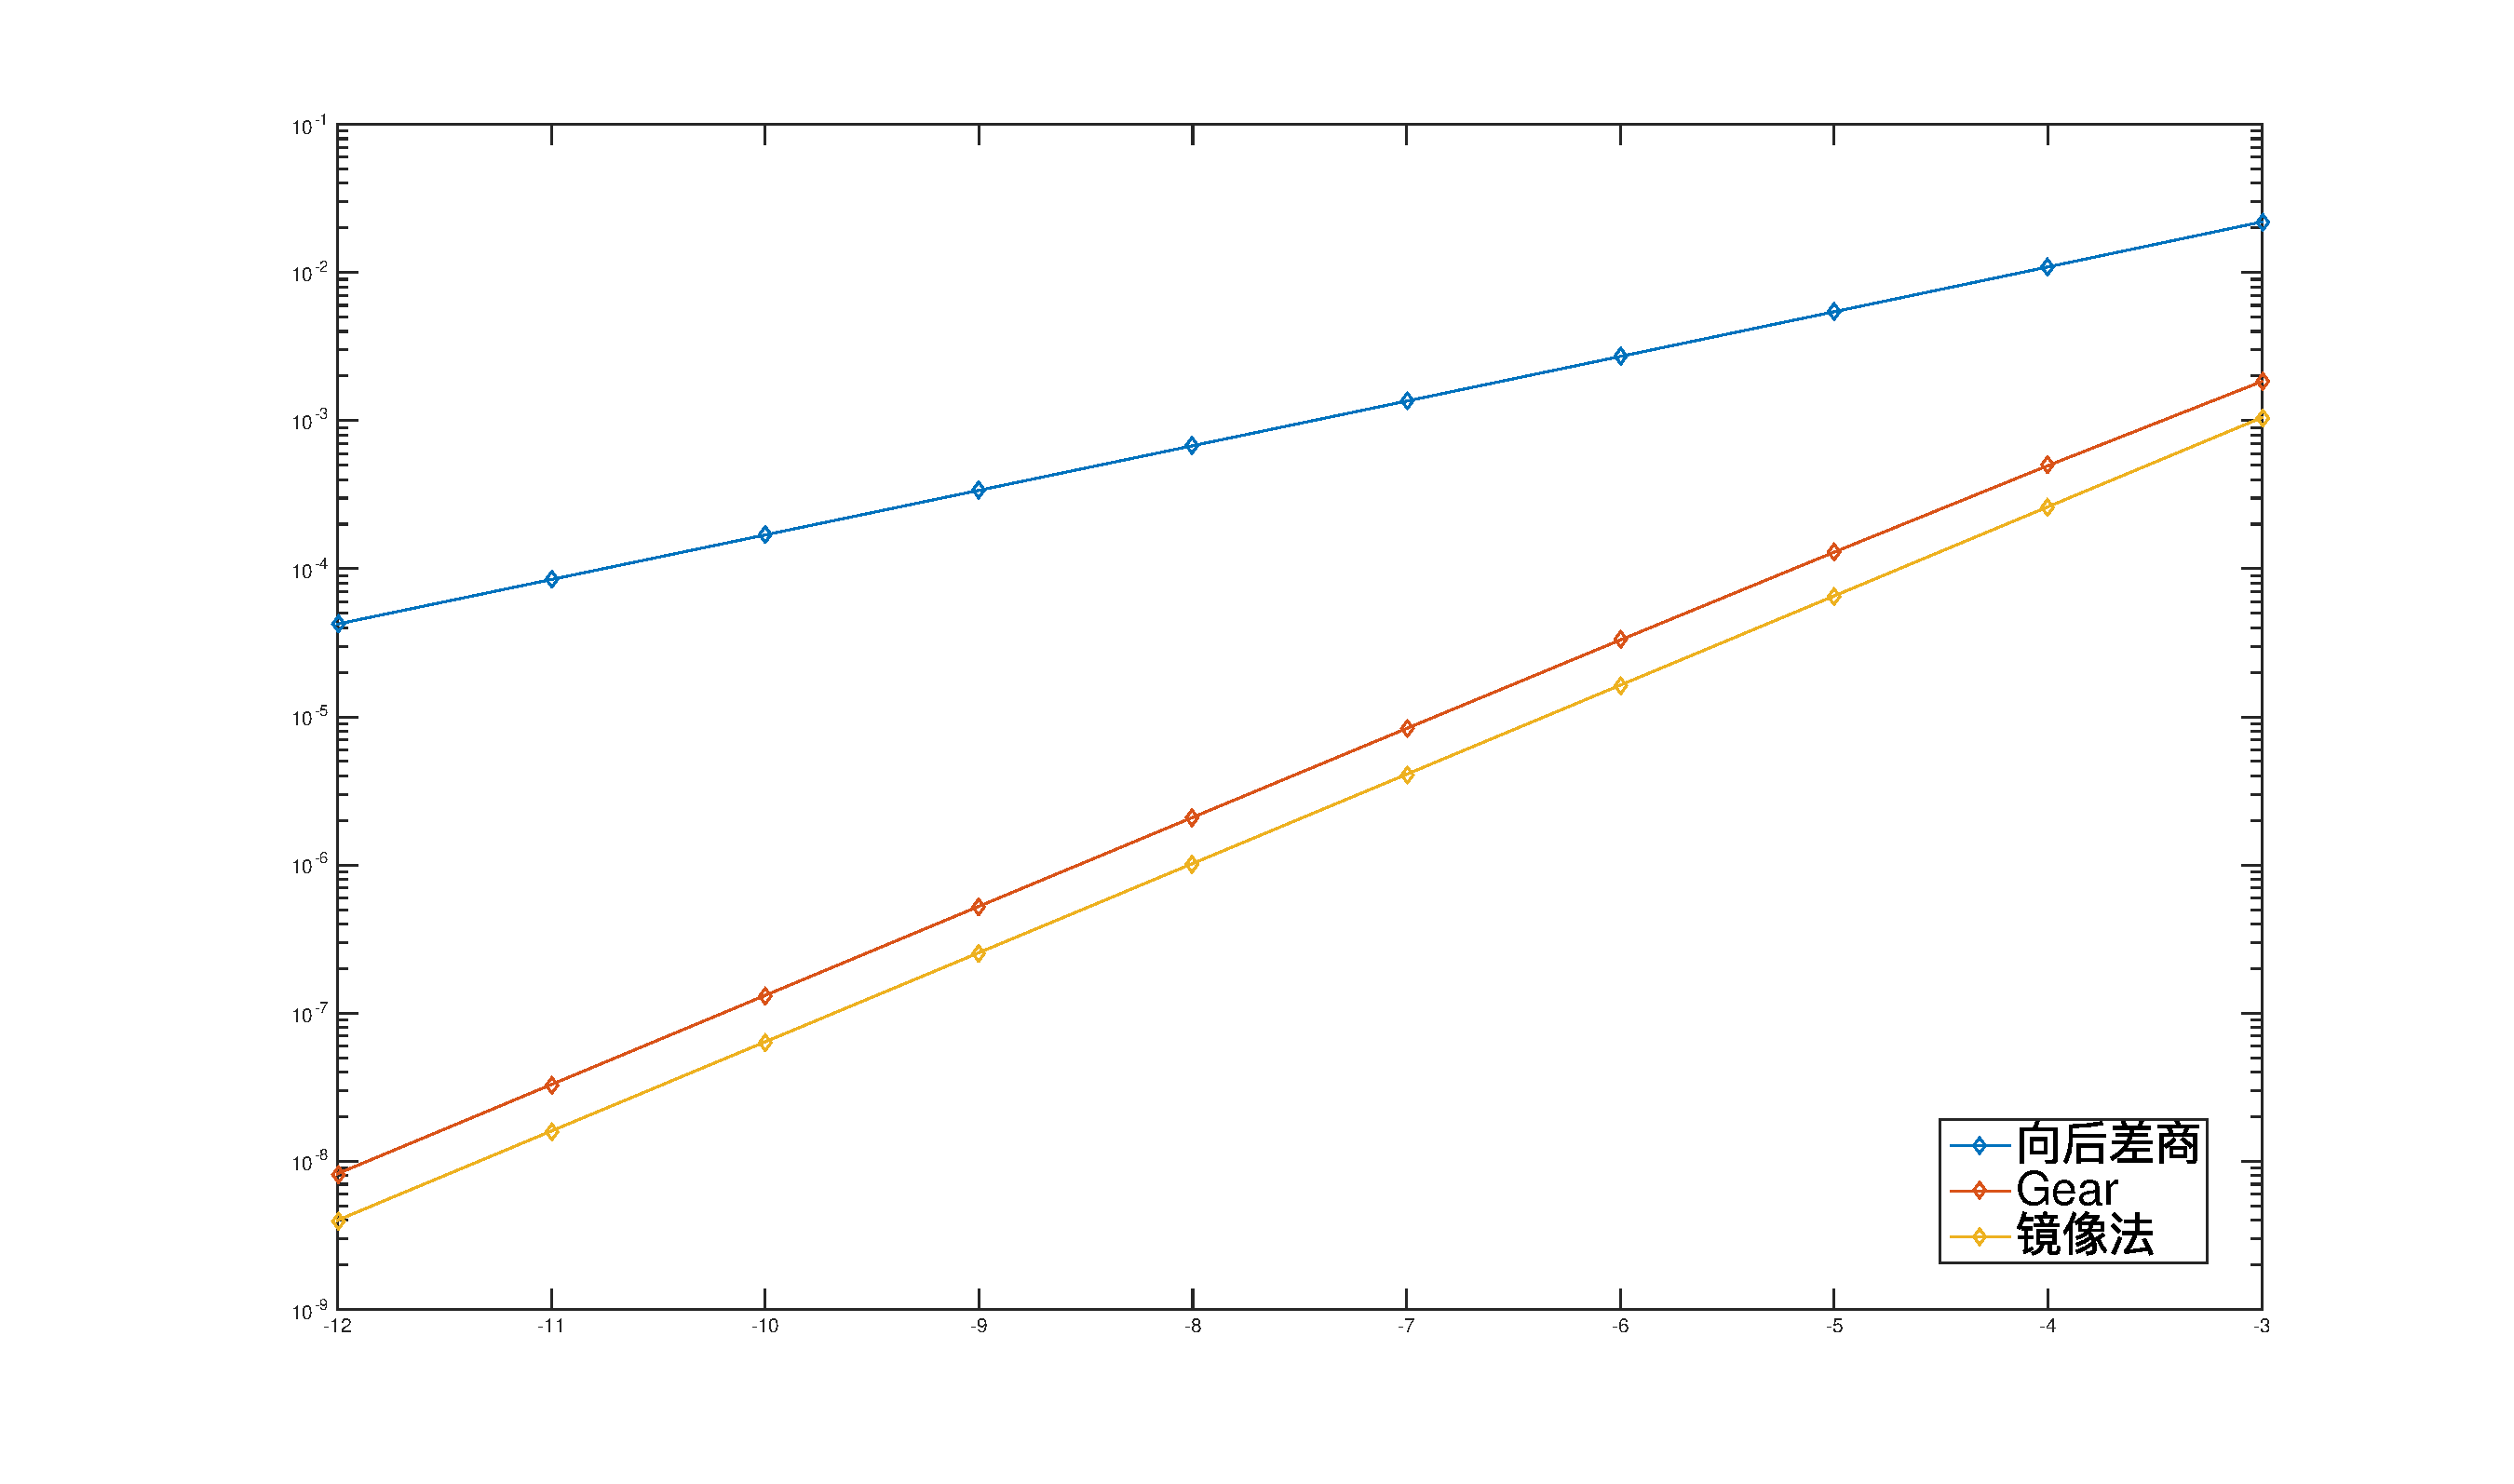
\includegraphics[width=5.5in]{H8_3_1.eps}}


\end{enumerate}






\end{enumerate}
\end{document}